\chapter{Sequential Logic}

\section{Introduction}

We will now analyze \textbf{sequential logic}. In addition to being dependend on the current input,
sequential logic is also dependend on the prior input (past state). We therefore say, sequential
logic has \textbf{memory}.

\section{Latches and Flip-Flops}
\subsection{SR Latch}

One of the simplest sequential circuits is the SR Latch, it can be built from either NOR
or NAND gates. The state of the SR Latch can be controlled through the $S$ (set) and the $R$ (reset) 
input.

\begin{figure}[h]
    \centering
    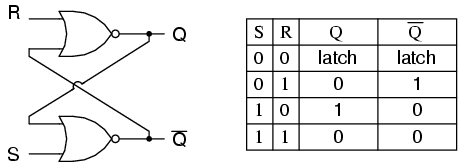
\includegraphics[width=10cm]{SR-Latch.png}
    \caption{SR Latch}
\end{figure}

The SR Latch has the simple but powerful functionality, that if both inputs $R$ and $S$ are $0$, $Q$
will keep the previous values. The circuit has \textbf{memory}.

\subsection{D Latch}

The limitation of the SR Latch is, that by giving an input on $S$ and $R$ not do we change the state,
we also decide when the state should change. We want to seperate these two actions. In addition we
also want to remove the state where both set and reset are active. The D Latch does exactly that.
\pagebreak

\begin{figure}[h]
    \centering
    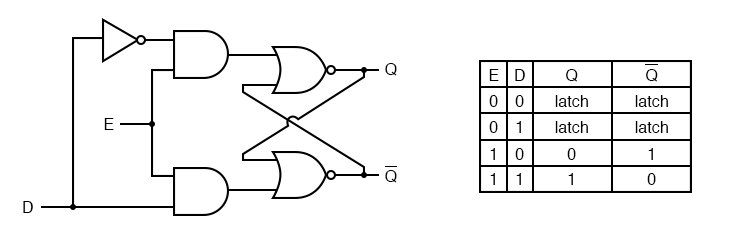
\includegraphics[width=13cm]{D-Latch.jpg}
    \caption{D Latch}
\end{figure}

A D Latch has two inputs, one data input $D$ and a clock input $E$ or $CLK$. Observe that when $E = 0$
the output will never change, only when $E = 1$ a new value is accepted from $D$. When $E = 1$, we
say that the latch is \textbf{transparent} and \textbf{opaque} otherwise.

\subsection{D Flip-Flop}

We notice that whenever $E$ is set to 1, a new input is accepted. This is not always desirable, we
often want a D Latch to only accept a input at the rising edge of the clock. We can combine two
D Latches to form a D Flip-Flop and achieve this desired behaviour.

\begin{figure}[h]
    \centering
    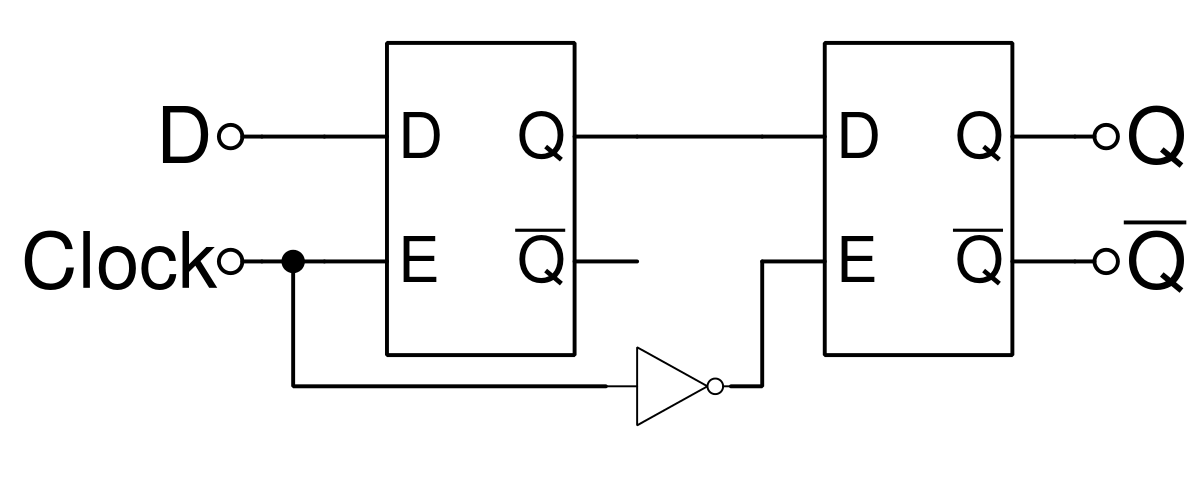
\includegraphics[width=11cm]{D-FlipFlop.png}
    \caption{D Flip-Flop}
\end{figure}

The first D Latche is calles the master and the second one is the slave. The functionality of the 
D Flip-Flop is essential for many digital designs and should be known by heart.

\begin{satz}[D Flip-Flop]
    A D Flip-Flop copies $D$ to $Q$ on the rising edge of the clock, and remembers its state at all
    other times.
\end{satz}

\subsection{Register}

An $N$-bit register is a bank of $N$ flip-flops that share a common clock signal. Registers are used
to save multiple bits of data and are a key building block of most sequential circuits.

\subsection{Enabled Flip-Flop}

An enabled flip-flop adds another input called $EN$ to determine whether data is loaded on the clock
edge or not. When $EN$ is true, it behaves like a normal D Flip-Flop otherwise it just retains its
current state.

\subsection{Resettable Flip-Flop}

A resettable flip-flop also adds another input called $RESET$. When $RESET$ is active, the resettable
flip-flop ignores $D$ and sets the output to 0. We make a difference between synchronously and 
asynchronously resettable flip-flops, the first only resets on the rising edge of the clock. Resettable
flip-flops are usefull, since at system startup we don't know in which state a flip-flop will be.

\section{Synchronous Logic Design}

In general, sequential circuits include all circuits that are not combinational, that is, those whos
outputs cannot be determined simply by looking at the current inputs.

A sequential circuit has a finite set of discrete states. A synchronous sequential circuit has a clock
input, whose rising edges indicate a sequence of times at which state transitions occure. The rules
of synchronous sequential circuit compositions are:

\begin{itemize}
    \item Every circuit element is either a register or a combinational circuit
    \item At least one circuit element is a register
    \item All registers receive the same clock signal
    \item Every cyclic path contains at least one register
\end{itemize}

Similarly, if a circuit is not synchronous, it is said to be asynchronous.

\section{Finite State Machines}

Finite state machines are synchronous sequential circuit with $k$ registers and $2^k$ possible states.
An FSM consists of two blocks of combinational logic, next state logic and output logic, and a register
that stores the state.

\begin{figure}[h]
    \centering
    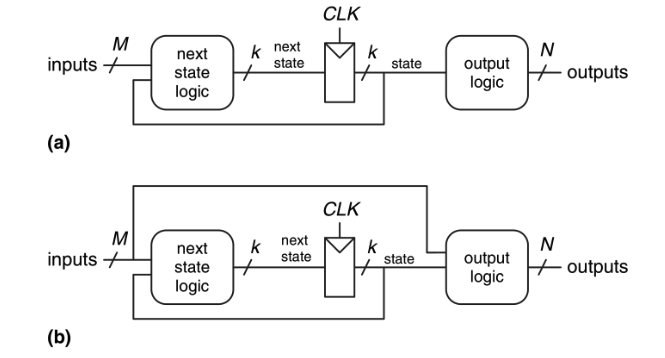
\includegraphics[width=10.8cm]{FSM.png}
    \caption{a) Moore Machine, b) Mealy Machine}
\end{figure}

There are two general classes of FSM, Moore Machines, where the output only depends on the current
state, and Mealy Machines, where the output depends on both the current state and the current inputs.

\subsection{Designing an FSM}

The design process for an FSM involves several different steps. Those steps are usually the same for
each FSM. Here we will look at this process for a Moore Machine:

\begin{itemize}
    \item Identify the inputs and outputs
    \item Sketch a state transition diagram
    \item Write a state transistion table
    \item Write a outpute table
    \item Select state encodings
    \item Write boolean equations for the next state and output logic
    \item Sketch the circuit schemantics
\end{itemize}

\begin{figure}[h]
    \centering
    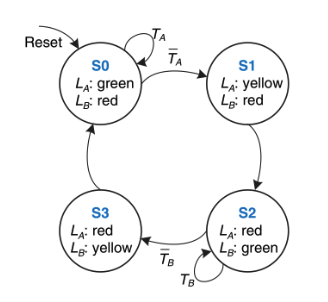
\includegraphics[width=8cm]{state-transition-diagram.png}
    \caption{State transition diagram of a stop light}
\end{figure}

\section{Timing of Sequential Logic}

When a clock rises, the output may start to change after the contamination delay and must definitely
settle to the final value within the propagation delay. For the circuit to sample its input correctly,
the input must be stable at least some time before the rising edge, setup time, and remain stable for
at least some time after the rising edge, hold time. The sum of setup and hold time is called the
aperture time of a circuit, during this time, the input must remain stable. The dynamic discipline
states that inputs of a synchronous circuit must be stable during the aperture time.

\subsection{Metastability}
As noted earlier, it is not always possible to guarantee that the input to a sequential circuit is 
stable during the aperture time. When a flip-flop samples an input that is changing during its aperture, 
the output $Q$ may momentarily take on a voltage between $0$ and $V_{DD}$ that is in the forbidden zone. 
This is called a metastable state.

\section{Parallelism}

The speed of a system is characterized by the latency and throughput of information moving thought it.
We define a \textbf{token} to be a group of inputs that are processed to produce a group of outputs. 
The \textbf{latency} of a system is the time required for one token to pass through the system from 
start to end. The \textbf{throughput} is the number of tokens that can be produced per unit time.


The throughput can be improved by processing several tokens at the same time. This is called 
parallelism, and it comes in two forms: spatial and temporal. With spatial parallelism, multiple 
copies of the hardware are provided so that multiple tasks can be done at the same time. With 
temporal parallelism, a task is broken into stages, like an assembly line. Those taks can be spread 
across stages, and if spread correctly, a different task will be in each stage at any given time so 
multiple tasks can overlap. Temporal parallelism is commonly refered to as pipelining.